\documentclass{article}
\usepackage{graphicx} % Required for inserting images
\usepackage[english]{babel}
\usepackage{amsmath}
\usepackage{amsfonts}
\usepackage{amsthm}
\usepackage{amssymb}
\usepackage{physics}
\usepackage[mathscr]{euscript}
\let\euscr\mathscr \let\mathscr\relax
\usepackage[scr]{rsfso}
\newcommand{\powerset}{\raisebox{.15\baselineskip}{\Large\ensuremath{\wp}}}

\usepackage{calligra}

\DeclareMathAlphabet{\mathcalligra}{T1}{calligra}{m}{n}
\DeclareFontShape{T1}{calligra}{m}{n}{<->s*[2.2]callig15}{}
\newcommand{\scriptr}{\mathcalligra{r}\,}
\newcommand{\bscriptr}{\pmb{\mathcalligra{r}}\,}

\usepackage{mathtools}


\numberwithin{equation}{section}
\numberwithin{figure}{section}

\newcommand{\vbh}[1]{\vb{\hat{#1}}}

\newcommand{\set}[1]{\{#1\}}
\newcommand{\FT}{\mathcal{F}}
\newcommand\perm[2][^n]{\prescript{#1\mkern-2.5mu}{}P_{#2}}
\newcommand\comb[2][^n]{\prescript{#1\mkern-0.5mu}{}C_{#2}}

\DeclareMathOperator{\spn}{span}

\renewcommand{\theequation}{Eq. \thesection.\arabic{equation}}

\DeclareMathOperator{\arccosh}{arcCosh}
\DeclareMathOperator{\arcsinh}{arcsinh}
\DeclareMathOperator{\arctanh}{arctanh}
\DeclareMathOperator{\arcsech}{arcsech}
\DeclareMathOperator{\arccsch}{arcCsch}
\DeclareMathOperator{\arccoth}{arcCoth} 

\makeatletter
\renewcommand*\env@matrix[1][*\c@MaxMatrixCols c]{%
  \hskip -\arraycolsep
  \let\@ifnextchar\new@ifnextchar
  \array{#1}}
\makeatother

\newtheorem{theorem}{Theorem}[section]
\newtheorem{corollary}{Corollary}[theorem]
\newtheorem{lemma}[theorem]{Lemma}
\title{PHYS 110A Homework 2}
\author{Siyu Chen}
\date{Summer 2023}

\begin{document}

\maketitle

\section{Problem 2.6}

\paragraph{Find the electric field a distance $z$ above the center of a flat circular disk of radius $R$ (Fig. 2.10) that carries a uniform surface charge $\sigma$. What does your formula give in the limit $R \to \infty$? Also check the case $z >> R$. \\}

Our geometry of the problem is:
\begin{figure}[!htb]
    \centering
   \begin{minipage}{0.48\textwidth}
     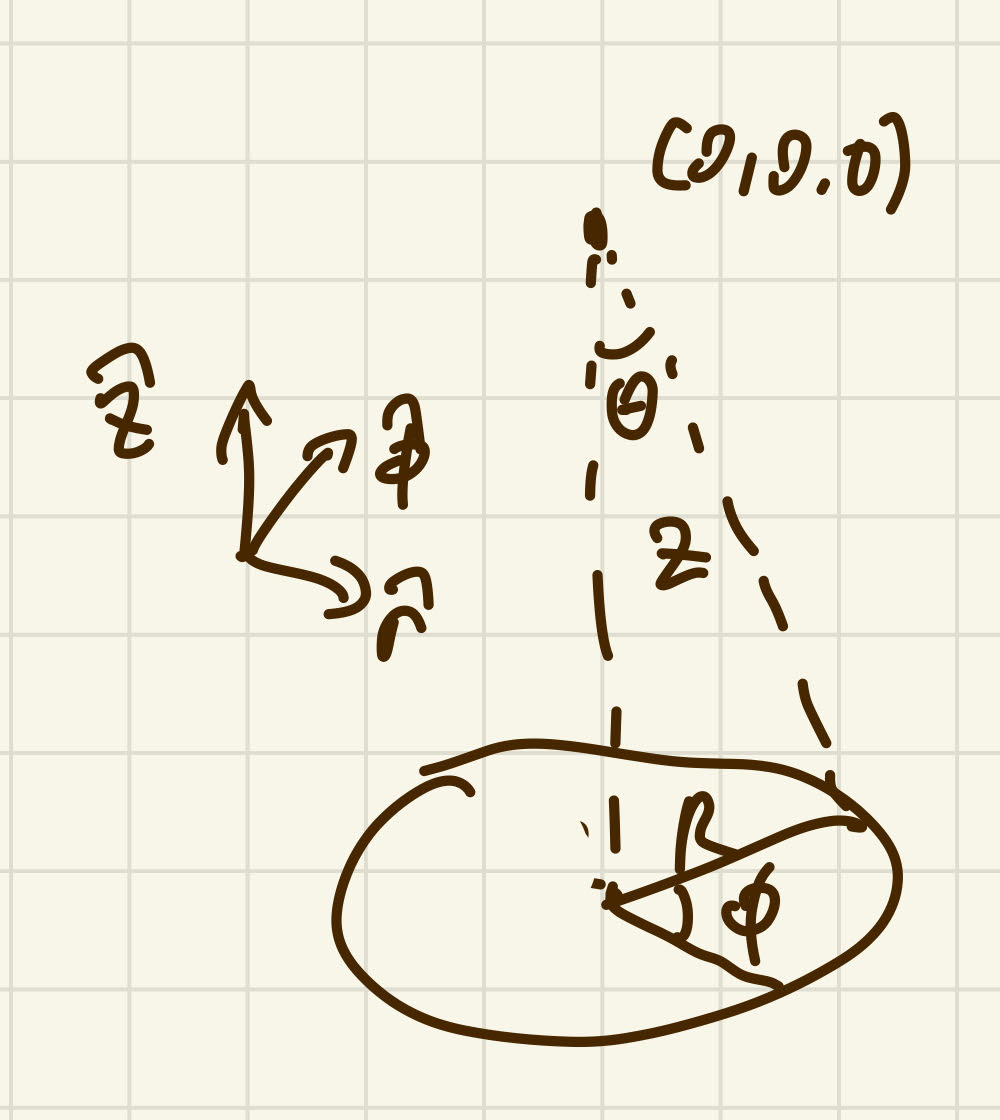
\includegraphics[width=0.8\linewidth]{hw/hw2/1.1.jpg}
     \caption{The disk of charge with point $z$ above its center}
   \end{minipage}
\end{figure}

The electric field if we define our charge distribution at $r'$ and our point $z$ away from center as the origin is given by the equation:

\begin{equation}
    \vb{E} = \frac{\sigma}{4 \pi \epsilon_0} \int_S \frac{1}{\scriptr^2} dr'  
\end{equation}

Since the cylindrical geometry, we can see that the electric field will be only be directed in the $z$ direction, since in the radial direction, the fields will cancel each other out. Therefore $\vb{E} = E_z \vbh{z}$. The expression for the $z$ component of our electric field is given by:

\begin{equation}
    E_z = E= \vb{E} \cos \theta =  \vb{E} \frac{z}{ \sqrt{z^2 + r^2}}
\end{equation}

since $\cos \theta = \frac{z}{ \sqrt{z^2 + r^2}}$, the adjacent over the hypotenuse. Now let's think about our definition of $\scriptr$. We can write:

\begin{equation}
    \scriptr = \sqrt{z^2 + r^2}
\end{equation}

Now let's write out our bounds of integration. We have to integrate over the circular surface of a disk, so $r$ goes from $0 \to R$, $\phi$, the angle around the disk, goes from $0 \to 2\pi$, and our collective $dr'$ becomes $dA = r dr d\phi$. We have our integral:

\begin{equation}
\begin{split}
    \vb{E} &= E_z \vbh{z} = \frac{\sigma}{4 \pi \epsilon_0} \int_S \frac{\cos \theta}{\scriptr^2} dr' \vbh{z} \\
     &= \frac{\sigma}{4 \pi \epsilon_0} \int_0^{2\pi} d\phi \int_0^R dr \frac{zr}{(z^2+r^2)^{3/2}} \\
     &= \frac{z \sigma}{4 \pi \epsilon_0} 2 \pi \lbrack \frac{1}{\sqrt{r^2 + z^2}} \rbrack^{0}_{R} \\
     &= \frac{\sigma}{2 \epsilon_0} (1 - \frac{z}{\sqrt{z^2 + R^2}})
    \end{split}
\end{equation}

we can see that as $R \to \infty$, $\vb{E} = \frac{\sigma}{2 \epsilon_0} \vbh{z}$, which is the expression for an infinite charge of sheet. At $z >> R$, we have $\vb{E} = 0$, which makes sense if $z$ is much further away than the radius of the charged disk.

\section{Problem 2.7}

\paragraph{Find the electric field a distance $z$ from the center of a spherical surface of radius $R$ (Fig. 2.11) that carries a uniform charge density $\sigma$. Treat the case $z < R$ (inside) as well as $z > R$ (outside). Express your answers in terms of the total charge $q$ on the sphere. \\}

The geometry of our problem is:

\begin{figure}[!htb]
    \centering
   \begin{minipage}{0.48\textwidth}
     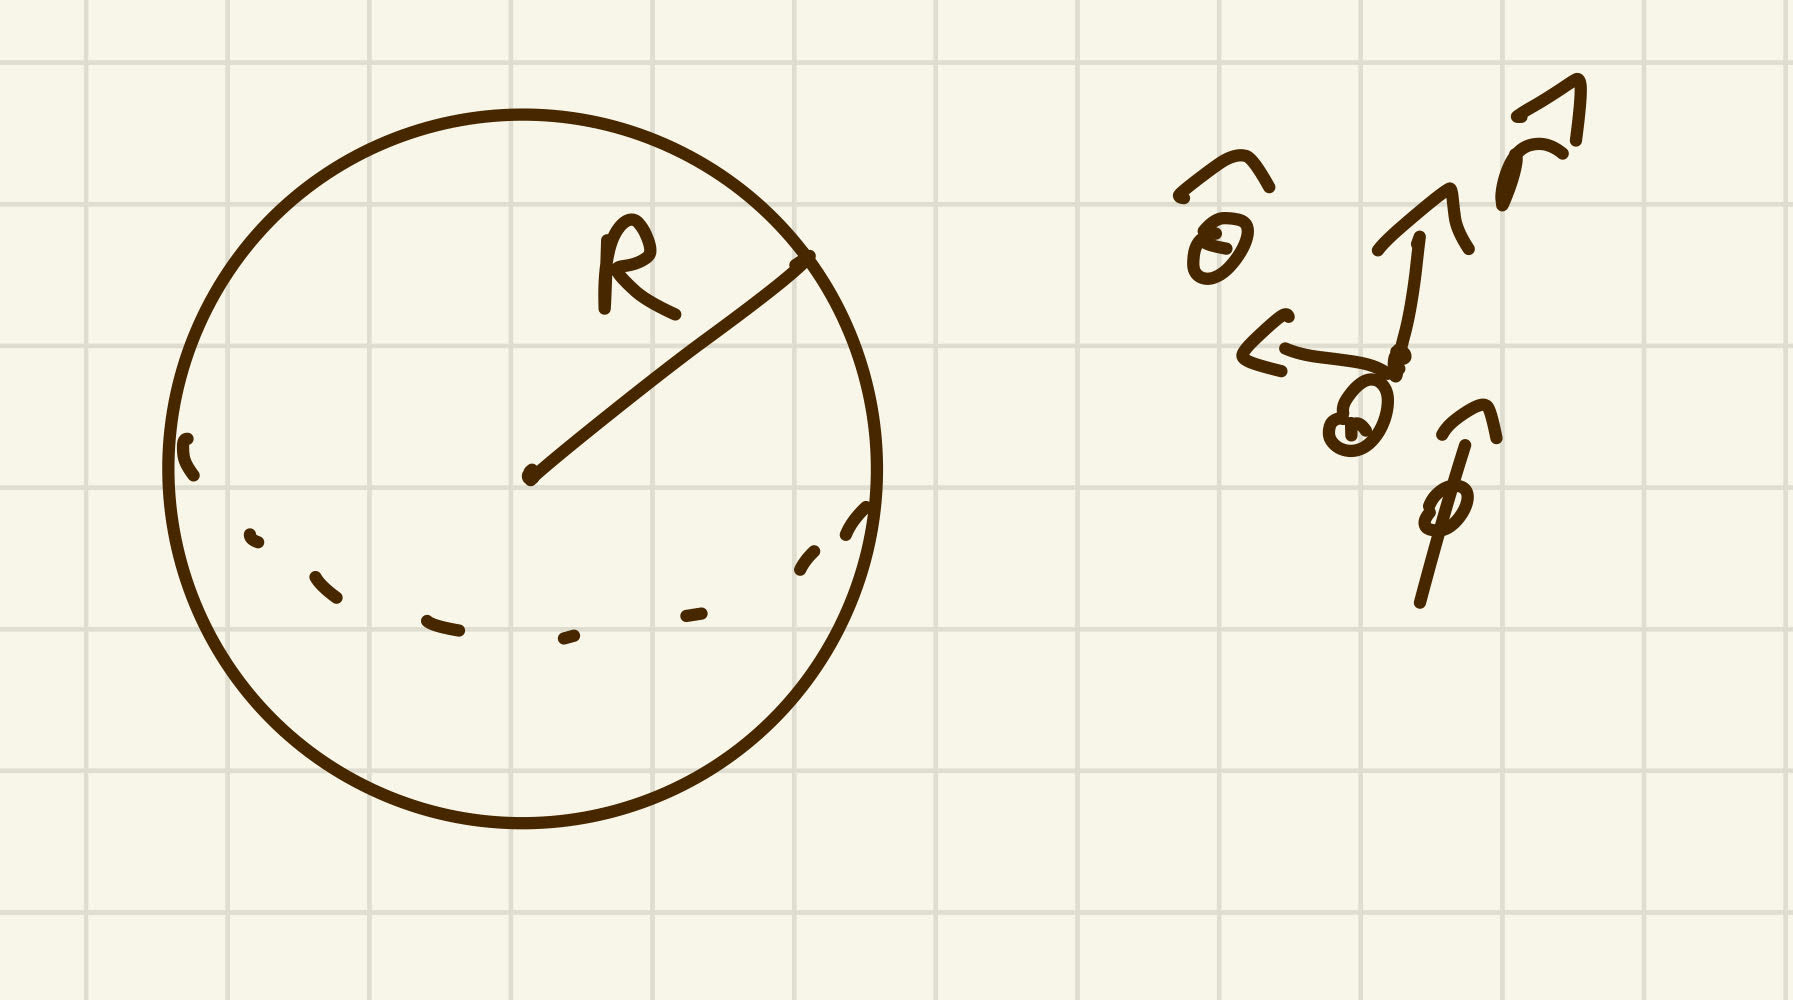
\includegraphics[width=1\linewidth]{hw/hw2/2.1.jpg}
     \caption{A uniform charge density solid sphere of radius $R$}
   \end{minipage}
\end{figure}

We can simply use Gauss's Law to treat this problem. Gauss's Law states that

\begin{equation}
    \oint_S \vb{E} \cdot d \vb{a} = \frac{q_{in}}{\epsilon_0}
\end{equation}

In all scenarios of this problem, since all electric field and the area vector are all in the positive radial direction, the integral is simply $E A$. In the case that $z < R$, $q_{in} = 0$ because all charges are on the surface, therefore $\vb{E} = 0$. Now consider outside the surface, from Eq. 2.1, we have:

\begin{equation}
    EA = \frac{q_{in}}{\epsilon_0}
\end{equation}

Consider the enclosed charge, we have enclosed the entire surface, so it is just $q$. Consider the area, it is just the area of the spherical Gaussian surface that we choose at $z$ away: $A = 4 \pi z^2$. We have

\begin{equation}
    \vb{E} = \frac{q}{4 \pi \epsilon_0 z^2} \vbh r
\end{equation}

\section{Problem 2.15}

\textbf{A thick spherical shell carries charge density}

\begin{equation*}
    \rho = \frac{k}{r^2} \quad ( a \leq r \leq b)
\end{equation*}

\paragraph{Find the electric field in the three regions: (i) $r < a$, (ii) $a < r < b$, (iii)
$ r > b$. Plot $\abs{E}$ as a function of $r$, for the case $b = 2a$. \\}

The geometry of our problem is:

\begin{figure}[!htb]
    \centering
   \begin{minipage}{0.48\textwidth}
     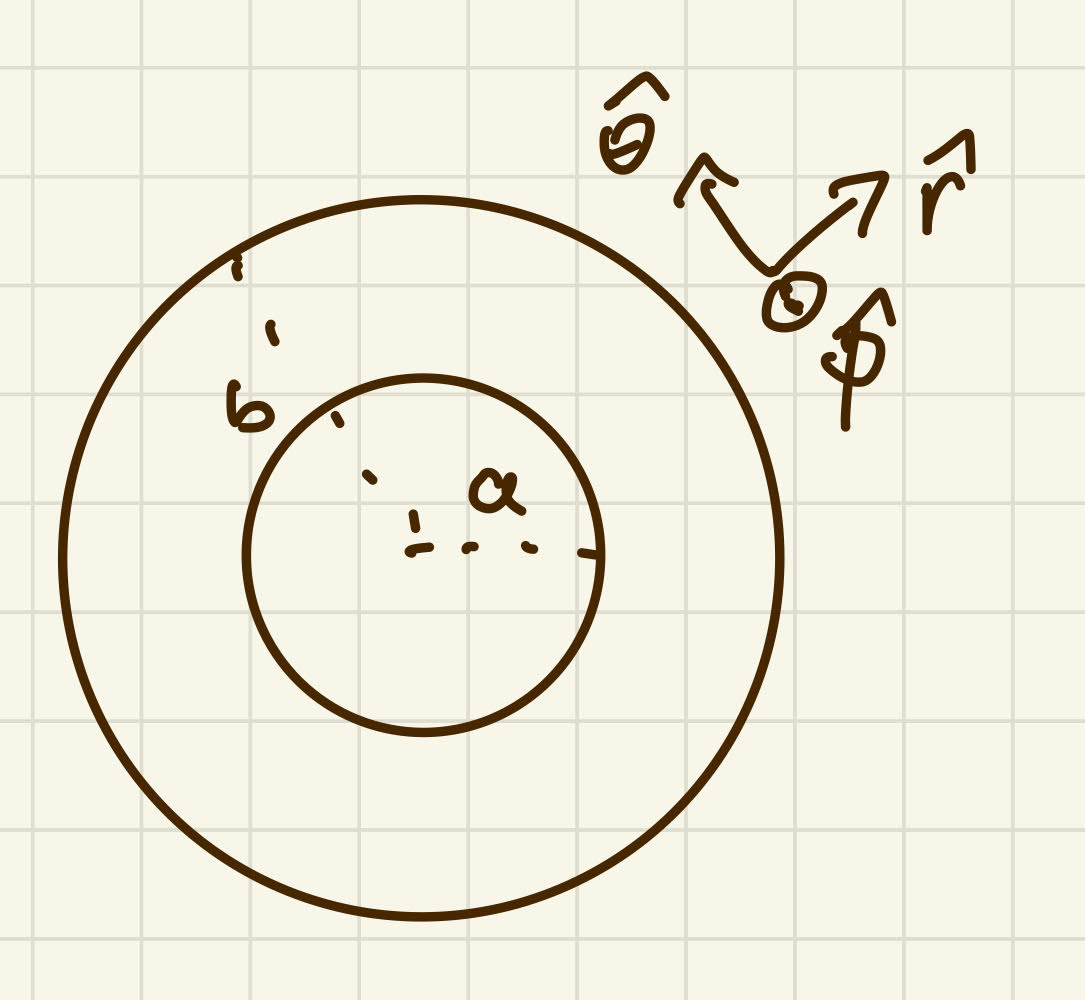
\includegraphics[width=.7\linewidth]{hw/hw2/3.1.jpg}
     \caption{The shell of charge between radius $a$ and $b$}
   \end{minipage}
\end{figure}

(i) The area inside the hollow part of spherical charge encloses no charge. By Gauss's Law:

\begin{equation}
    \oint_S \vb{E} \cdot d \vb{a} = EA = \frac{q_{in}}{\epsilon_0} = 0 \Rightarrow \vb{E}_{1} = 0
\end{equation}

The electric field inside this region is $0$. \\

(ii) The area in between $a, b$ also has electric field in the radial direction due to its symmetry. The enclosed charge is given by:

\begin{equation}
    q_\text{in} = \int dq = \int \rho d\tau
\end{equation}

The volume $d\tau = 4 \pi r'^2 dr'$, and the charge density $\rho = \frac{k}{r'^2}$ inside this region.

\begin{equation}
    q_\text{in} = \int_a^r 4 \pi r'^2 \frac{k}{r'^2} dr' = 4 \pi k (r - a)
\end{equation}

The area of our Gaussian surface is a function of $r$ as well. $A = 4 \pi r^2$. So in Gauss's Law, we have

\begin{equation}
    E = \frac{q_{in}}{\epsilon_0 A} = \frac{4 \pi k(r-a)}{\epsilon_0 4 \pi r^2} = \frac{k}{\epsilon_0} \frac{(r-a)}{r^2}
\end{equation}

and of course, the vector $\vb{E}$ is just the above expression with $\vbh r$. \\

(iii) for the case $r > b$, we have enclosed the entirety of our spherical shell. So $q_{in} = q$. To find $q$, we use the same method as (3.3) except our bound of integration has changed to $a \to b$ to cover the entire shell and not $a \to r$:

\begin{equation}
    q = \int \rho d \tau = \int_a^b 4 \pi r'^2 \frac{k}{r'^2} dr' = 4 \pi k (b-a)
\end{equation}

The electric field is once again given by:

\begin{equation}
    E = \frac{q}{\epsilon_0 A} = \frac{k(b-a)}{r^2 \epsilon_0},\quad  \vb{E} = E \vbh r
\end{equation}

Let's organize our values of electric field:

\begin{equation}
    \vb{E} = \begin{cases}
        0 \quad &( r \leq a) \\
        \frac{k}{\epsilon_0} \frac{(r-a)}{r^2} \vbh r & (a \leq r \leq b) \\
        \frac{k(b-a)}{r^2 \epsilon_0} \vbh r & (b \leq r)
    \end{cases}
\end{equation}

(iv) To better graph this at $b = 2a$, we can compute some key points of electric field and compute its derivative for the middle part:

\begin{equation}
\begin{split}
    E(a) &= 0 \\
    \frac{dE}{dr} &= \frac{k}{\epsilon_0}(- r^{-2} + 2a r^{-3}) \quad (a \leq r \leq 2a) \\
    \frac{dE}{dr} \rvert_{2a} &= 0 \\
    E(2a) &= \frac{ka}{\epsilon_0 4a^2}
\end{split}
\end{equation}

our graph is:\begin{figure}[!htb]
    \centering
   \begin{minipage}{0.48\textwidth}
     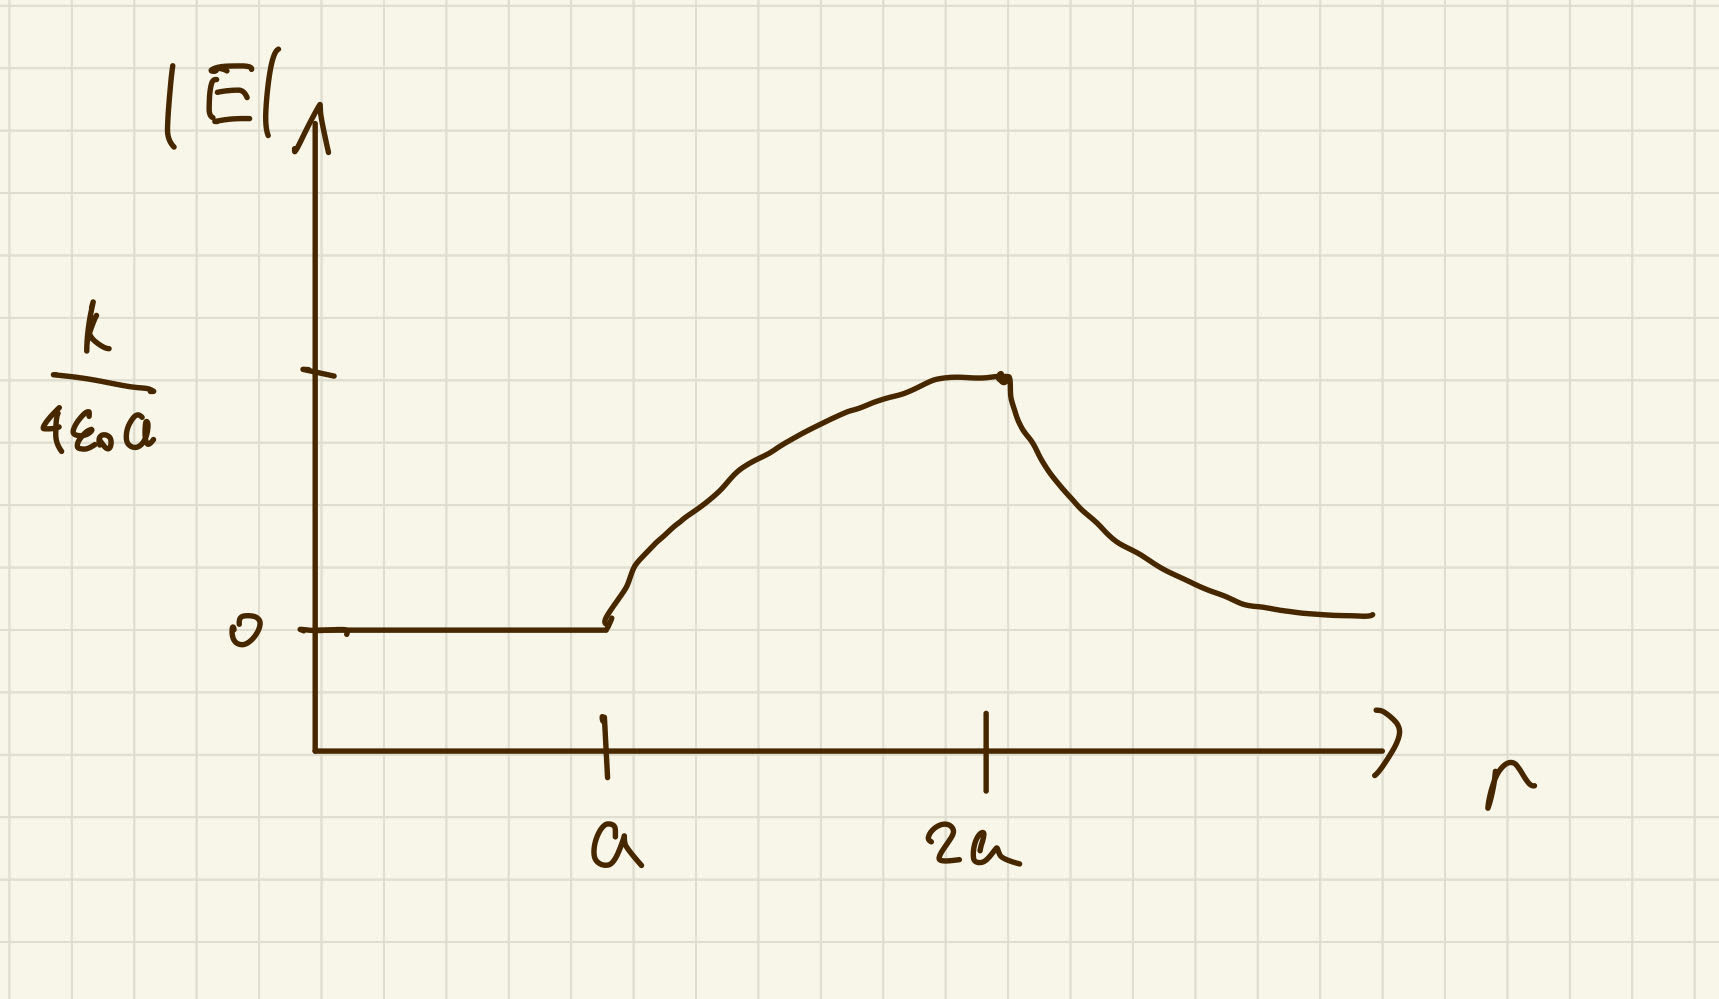
\includegraphics[width=1.2\linewidth]{hw/hw2/3.2.jpg}
     \caption{$\abs{E}$ as a function of $r$}
   \end{minipage}
\end{figure}

The function of $\abs{E}$ is $0$ for $r<a$, for the region in between $a, b$, it increases to a maximum at $r = 2a$, and approaches $0$ as $r \to \infty$
 
\section{Problem 2.20}

\paragraph{One of these is an impossible electrostatic field. Which one?}

\begin{equation*}
    \begin{split}
        (a) \vb{E} &= k [xy \vbh x + 2 yz \vbh y + 3xz \vbh z]; \\
        (b) \vb E &= k [y^2 \vbh x + (2xy + z^2) \vbh y + 3yz \vbh z].
    \end{split}
\end{equation*}

Since we know that $\curl \vb E = 0$, we just need to take the curl of (a) and (b) and see if they are zero.

\begin{equation}
    \curl \vb E_a = k ( -2y \vbh x - z \vbh y - x \vbh z) \not = 0
\end{equation}

This electric field should not be possible and that is our answer. Let's just verify that the other electric field is possible.

\begin{equation}
    \curl \vb E_b = k (2z - 2z) \vbh x - (0 - 0 ) \vbh y + ( 2y - 2y) \vbh z = 0
\end{equation}

and this is a possible electric field.

\section{Problem 2.21}

\paragraph{Find the potential inside and outside a uniformly charged solid sphere whose radius is $R$ and whose total charge is $q$. Use infinity as your reference point. Compute the gradient of $V$ in each region, and check that it yields the correct field. Sketch $V (r)$. \\}

We can compute our potential as $V = - \int \vb E \cdot d \vb r$. So we first have to find our electric fields and we can do that by Gauss's Law. First consider the region inside the sphere. Let's find $q_{in}$ first:

\begin{equation}
    q_\text{in} = \rho \int d \tau = \rho \frac{4}{3} \pi r^3 \quad (r < R)
\end{equation}

Then in Gauss's Law, our Gaussian surface would be a spherical surface with radius $r$, and its area is $A = 4 \pi r^2$. Since everything is in radial direction only, we can write:

\begin{equation}
    \vb E = E_r \vbh r = \frac{q_{in}}{A \epsilon_0} \vbh r = \frac{\rho}{3 \epsilon_0} \vb r \quad (r < R)
\end{equation}

The electric field outside of the sphere would just be the same from a point charge of $q$ at the center of the sphere. We can show this by Gauss's Law that $E = q / A \epsilon_0$ and $A \epsilon_0 = 4 \pi r^2 \epsilon_0 = r^2 / k$ and we have $E = kq / r^2$

\begin{equation}
    \vb E = \frac{q}{4\pi \epsilon} \frac{1}{r^2} \vbh r \quad (r > R)
\end{equation}

Then let's compute the potential outside of the sphere, with infinity at 0:

\begin{equation}
    V(r) = V(r) - V( \infty) = - \int_{\infty}^r \vb E \cdot d \vb r' = - kq \int^r_\infty \frac{dr'}{r'^2} =  kq \frac{1}{r'} \rvert^r_\infty = \frac{kq}{r}
\end{equation}

Then let's compute the potential inside the sphere:

\begin{equation}
\begin{split}
    V(r) - V(R) &= - \int_R^r \vb E \cdot d \vb r' = - \frac{\rho}{3 \epsilon_0}\int_R^r  r dr \\
    V(r) &= - \frac{6}{\epsilon_0} r'^2 \rvert^r_R + V(R) = \frac{\rho}{6 \epsilon_0} (R^2 - r^2) + \frac{kq}{R}
\end{split}
\end{equation}

We have both $\rho$ and $q$, let's just write $\rho$ as $\rho = q \frac{3}{4\pi R^3}$. Organizing our results, we have:

\begin{equation}
    V (r) = \begin{cases}
        \frac{kq}{2R^3} (R^2 - r^2) + \frac{kq}{R} \quad \quad &r \leq R \\
        \frac{kq}{r} \quad \quad &r \geq R
    \end{cases}
\end{equation}

The gradient of the two regions are just given by their component of $\vbh r$ partial derivatives as our function is only a function of $r$.

\begin{equation}
    \grad V_\text{in} = \frac{\partial}{\partial r} \frac{kq}{2R^3} (R^2 - r^2) + \frac{kq}{R}= -\frac{kqr}{R^3} \vbh r
\end{equation}

we can see that this is the correct result by verifying that it is the negative of our electric field, which is given by Gauss's Law:

\begin{equation}
    \vb E_\text{in} = \frac{q_{\text{in}}}{\epsilon_0 A}\vbh r = \frac{kq}{\epsilon_0 4 \pi r^2} \frac{\tau_\text{in}}{\tau}\vbh r =  \frac{kq}{\epsilon_0 4 \pi r^2} \frac{r^3}{R^3} \vbh r= \frac{kqr}{R^3}\vbh r
\end{equation}

The outer region gradient is:

\begin{equation}
    \grad V_\text{out} = \frac{\partial}{\partial r} \frac{kq}{r} = - \frac{kq}{r^2} \vbh r
\end{equation}

which is indeed the negative of our electric field from Eq. 5.3, which states:

\begin{equation}
    \vb E_\text{out} = \frac{kq}{r^2} \vbh r
\end{equation}

To graph it better, $V(0) = kq (\frac{1}{2R} + \frac{1}{R}) = \frac{3}{2}kqR$

\begin{figure}[!htb]
    \centering
   \begin{minipage}{0.48\textwidth}
     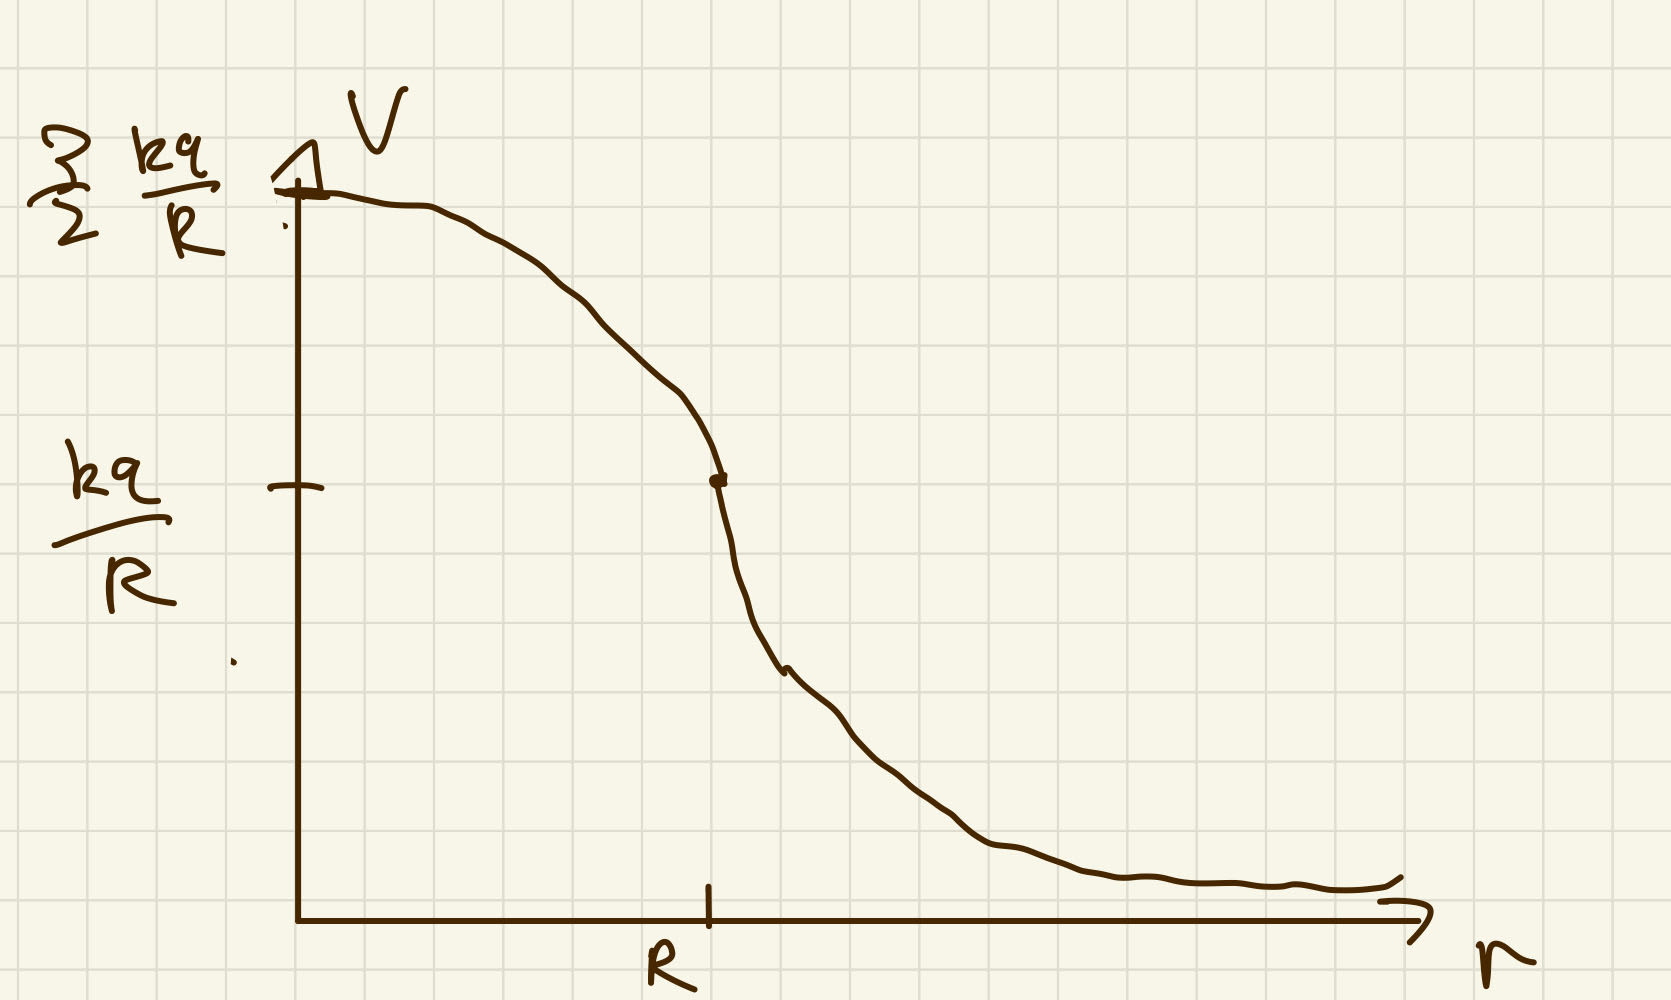
\includegraphics[width=1.2\linewidth]{hw/hw2/5.1.jpg}
     \caption{$V$ as a function of $r$}
   \end{minipage}
\end{figure}

The function decreases as $-r^2$ until $R$ and then approaches $0$ as $r \to \infty$.


\section{Problem 2.23}

\paragraph{For the charge configuration of Prob. 2.15, find the potential at the center, using infinity as your reference point. \\}

The charge configuration of 2.15 is that of the spherical shell between radius $a$ and $b$. The summary of the results we obtained for the electric field is the following:

\begin{equation}
\begin{split}
        \vb E_{\text{in}} &= 0 \quad \quad \quad \quad \quad \quad ( r \leq a) \\
        \vb E_{\text{shell}} &= \frac{k}{\epsilon_0} \frac{(r-a)}{r^2} \vbh r  \quad \quad (a \leq r \leq b) \\
        \vb E_{\text{out}} &= \frac{k(b-a)}{r^2 \epsilon_0} \vbh r  \quad \quad (b \leq r)
\end{split}
\end{equation}

Let's use infinity as $V(\infty) = 0$, we have to find the potential of $V(0)$. Using the identity that $V(a)-V(b) = - \int^a_b \vb E \cdot d \vb r$, we have:

\begin{equation}
    \begin{split}
        V(0) &= V(b) - V(\infty) + V(a) - V(b) + V(0) - V(a) \\
        &= - \int^b_\infty \vb E_{\text{out}} \cdot d \vb r' - \int^a_b \vb E_{\text{shell}} \cdot d \vb r' - \int^0_a \vb E_{\text{in}} \cdot d \vb r' \\
        &= -\frac{k}{\epsilon_0} (b-a) \int^b_\infty \frac{dr'}{r'^2} - \frac{k}{\epsilon_0} \int^a_b (\frac{1}{r} - \frac{a}{r'^2}) dr' + 0 \\
        &= \frac{k}{\epsilon_0} (b-a) (\frac{1}{b} - \frac{1}{\infty}) - \frac{k}{\epsilon} \lbrack \ln \abs{\frac{a}{b}} + (1 - \frac{a}{b}) \rbrack \\
        &= \frac{k}{\epsilon_0} (b-a) (\frac{1}{b} - \frac{1}{b}) - \frac{k}{\epsilon_0} \ln \abs{\frac{a}{b}} \\
        V(0) &= \frac{k}{\epsilon_0} \ln \abs{\frac{b}{a}}
    \end{split}
\end{equation}

and that is our desired expression for the potential at the center.


\section{Problem 2.26}

\paragraph{A conical surface (an empty ice-cream cone) carries a uniform surface charge $\sigma$. The height of the cone is $h$, as is the radius of the top. Find the
potential difference between points $a$ (the vertex) and $b$ (the center of the top). \\}

The geometry of our problem is given by the following, note: in my sketch, I labeled the height $h$ as $H$ and the integration variable $h'$ as $h$.

\begin{figure}[!htb]
    \centering
   \begin{minipage}{0.48\textwidth}
     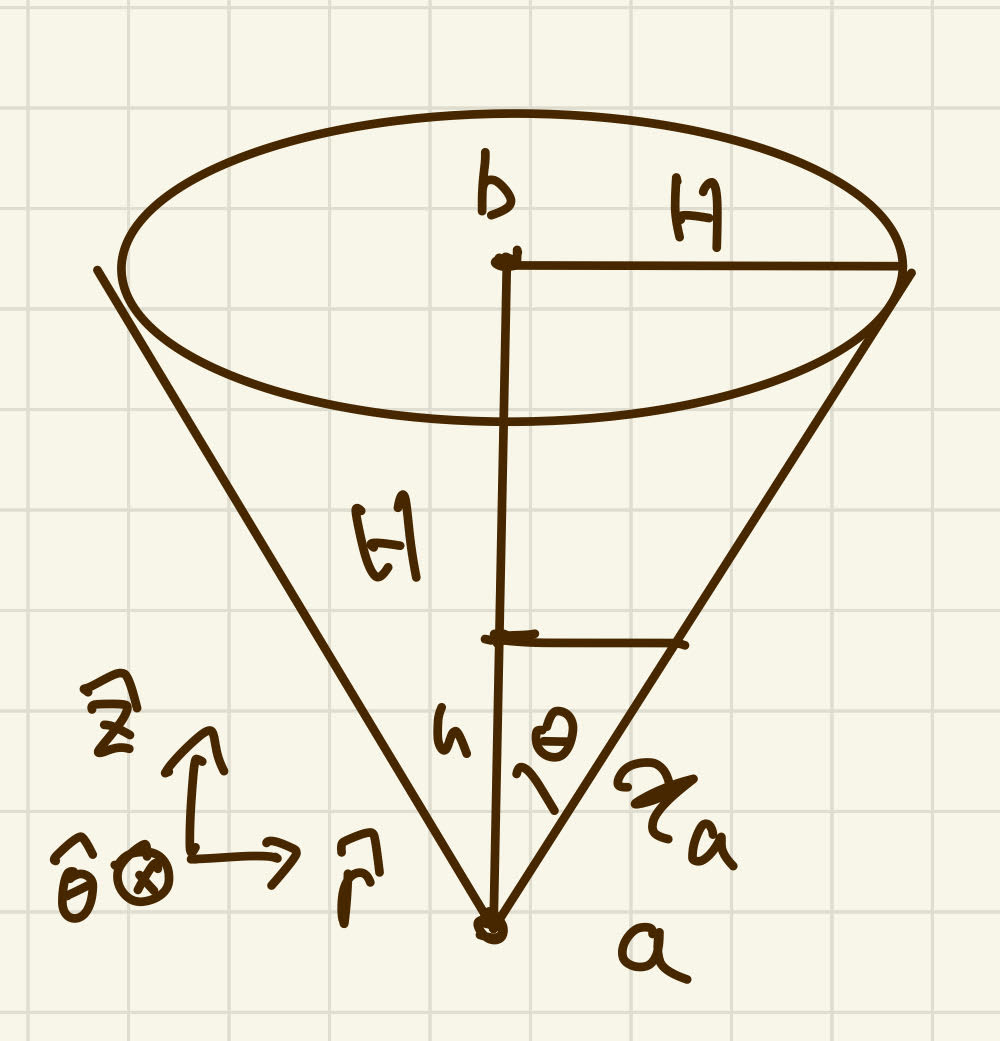
\includegraphics[width=1\linewidth]{hw/hw2/7.1.jpg}
     \caption{The conic surface of radius $h$ and height $h$}
   \end{minipage}
\end{figure}

With definition of $V(\infty) = 0$, we can simply use the formula

\begin{equation}
    V(a) = \int_S \frac{k}{\scriptr(a)}dq
\end{equation}

The geometry of the charge distribution is interesting. We have $dq = \sigma dA$. To consider our $dA$, we must be careful. In a conic surface

\begin{equation}
    dA = 2\pi r \frac{dh'}{\cos \theta}
\end{equation}

so that we are not integrating tiny cylinders but actually integrating along the hypotenuse. We are given that $r = h$, therefore we know that $\theta = \pi /4 $ and $\cos \theta = \sqrt{2}$. We have:

\begin{equation}
    dA = \sqrt{2} \pi h' dh'
\end{equation}

Now, we have to find the $\scriptr$ as a function of our points $a$ and $b$. $\scriptr(a)$ is relatively simpler, since it is at the vertex, the distance between it and all points on the conic surface is just the length of the hypotenuse, we have:

\begin{equation}
    \scriptr(a) = \frac{h}{\cos \theta} = \frac{h}{\sqrt{2}}
\end{equation}

Now we consider $\scriptr(b)$, it is more complicated. The distance is given by the hypotenuse of a right triangle with $h - h'$, the radius of the base of our conic surface as we integrate, at the base and $h'$, the height as we integrate our cone, as its height. We have:

\begin{equation}
    \scriptr(b) = \sqrt{(h-h')^2 + h'^2} = \sqrt{h^2 - 2hh' + 2h'^2}
\end{equation}

$h$ and $h'$ is truly one of the notations of all time. Moving on, we can write our potential difference as:

\begin{equation}
    V(b) - V(a) = \int_S \frac{k}{\scriptr(b)} dq - \int_S \frac{k}{\scriptr(a)} dq
\end{equation}

let's evaluate $V(a)$ first. We have

\begin{equation}
    V(a) = k \sigma \int_S \frac{dA}{\scriptr(a)} = k \sigma \sqrt{2}^2 \pi \int_0^h \frac{h' dh'}{h'} = 2\pi k \sigma h
\end{equation}

let's evaluate $V(b)$ next. We have:

\begin{equation}
\begin{split}
    V(b) &= k \sigma \int_S \frac{dA}{\scriptr(b)} = k \sigma \sqrt{2} \pi \int_0^h \frac{h' dh'}{\sqrt{h^2 - 2hh' + 2h'^2}} \\
    &= \frac{\arcsinh 1}{\sqrt{2}} h k \sigma \sqrt{2} \pi = \ln(1+\sqrt{2}) hk \sigma \pi
\end{split}
\end{equation}

and our positive potential difference, since $V(a) > V(b)$, is:

\begin{equation}
    V(a) - V(b) = k \sigma \pi h \left[ 2 - \ln(1 + \sqrt{2}) \right]
\end{equation}

\section{Problem 2.30}

\textbf{Following equations from Griffiths are relevant to this question:}

\begin{equation*}
    \vb E_{\text{above}} - \vb E_{\text{below}} = \frac{\sigma}{\epsilon_0} \vbh n \tag{Eq. 2.33, Griffiths}
\end{equation*}

\begin{equation*}
    V_{\text{above}} = V_{\text{below}} \tag{Eq. 2.34, Griffiths}
\end{equation*}

\begin{equation*}
    \frac{\partial V_{\text{above}}}{\partial n} -  \frac{\partial V_{\text{below}}}{\partial n} = - \frac{\sigma}{\epsilon_0} \tag{Eq. 2.36, Griffiths}
\end{equation*}

\paragraph{(a) Check that the results of Exs. 2.5 and 2.6, and Prob. 2.11, are consistent with Eq. 2.33.\\}

(i) Ex 2.5 derives that for an infinite charged sheet, the electric field is given by:

\begin{equation}
    \vb E = \frac{\sigma}{2 \epsilon_0} \vbh n'
\end{equation}

We label this $\vbh n'$ for Eq. 8.1 to distinguish it from the normal vector in Eq. 2.33 that we are trying to verify. In the context of Ex 2.5, the normal vector $\vbh n'$ points to two opposite directions that the sheet is pointed at depending on which region relative to the sheet we consider. In the definitions of Eq. 2.33, let's define one side of the infinite sheet as the "above side". We can see that $\vbh n' = \vbh n$ for the above side, and $\vbh n' = - \vbh n$ for the below side. We have that

\begin{equation}
    \vb E_{\text{above}} - \vb E_{\text{below}} = \frac{\sigma}{2 \epsilon_0} \vbh n - \frac{\sigma}{2 \epsilon_0} (- \vbh n) =  \frac{\sigma}{\epsilon_0} \vbh n
\end{equation}

and that it does satisfy Eq. 2.33. \\

(ii) Ex. 2.6 derives that with two infinite charge sheets of $\pm\sigma$ some distance apart, with the positive sheet on the left and negative sheet on the right, the region to the left and right side of the electric field has $\vb E = 0$, and the region in between the two sheets has electric field:

\begin{equation}
    \vb E_{\text{center}} = \frac{\sigma}{\epsilon_0} \vbh n'
\end{equation}

where $\vbh n'$ points toward the right. Let's define in the context of Eq. 2.33 that $\vbh n = \vbh n'$ and the right side is considered "above" side. For the left, positive sheet:

\begin{equation}
    \vb E_{\text{above}} - \vb E_{\text{below}} = \vb E_{\text{center}} - \vb E_{\text{left}} = (\frac{\sigma}{\epsilon_0} - 0) \vbh n = \frac{\sigma}{\epsilon_0}\vbh n
\end{equation}

We can see that this satisfies Eq. 2.33. For the right, negative sheet, the charge distribution is $- \sigma$, and still, the right side is above side.

\begin{equation}
    \vb E_{\text{above}} - \vb E_{\text{below}} = \vb E_{\text{right}} - \vb E_{\text{center}} = (0 - \frac{\sigma}{\epsilon_0}) \vbh n = - \frac{\sigma}{\epsilon_0} \vbh n
\end{equation}

We can see that this satisfies Eq. 2.33. as well.

(iii) Problem 2.11 is the same problem as 2.7, but explicitly asking us to do it with Gauss's Law, which we have done in this homework. The result from the problem states that for a spherical surface of radius $R$ and charge $q$ and uniform charge density:

\begin{equation}
\begin{split}
        \vb E_{\text{in}} &= 0 \\
        \vb E_{\text{out}} &= \frac{kq}{r^2}
\end{split}
\end{equation}

We are considering the electric field just outside our surface, so $r = R$ still, $\vb E_{\text{above}} = \frac{kq}{R^2} \vbh r$. We can define $\vbh r = \vbh n$ to be our above side. We can get the following expression:

\begin{equation}
    \vb E_{\text{above}} - \vb E_{\text{below}} = \vb E_{\text{out}} - \vb E_{\text{in}} = \vb E_{\text{out}} 
\end{equation}

The surface also has uniform charge density $\sigma = q / A = \frac{q}{4\pi R^2}$. We can see that the difference is just the out going radial electric field above the sphere.

\begin{equation}
    \vb E_{\text{above}} - \vb E_{\text{below}}= \frac{kq}{R^2} \vbh n = \frac{1}{4\pi \epsilon_0} \frac{4\pi R^2 \sigma}{R^2} \vbh n = \frac{\sigma}{\epsilon_0} \vbh n
\end{equation}

\paragraph{(b) Use Gauss’s law to find the field inside and outside a long hollow cylindrical tube, which carries a uniform surface charge $\sigma$. Check that your result is consistent with Eq. 2.33. \\}

Using cylindrical coordinate, our cylinder has radius $\rho$, length $l$, we can see that all outgoing electric field is in the $\vbh \rho$ direction, which is the same direction as the $d \vb a$, area segment vector. Therefore $ \vb E \cdot d \vb a = E da$. We can also see that, inside the cylindrical tube, we enclose no charge, therefore by Gauss's Law, we can see that:

\begin{equation}
    \vb E_{\text{in}} = 0
\end{equation}

For the electric field outside the cylindrical tube, we see that the enclosed charge is just $q$. We also see that the area of our Gaussian surface is a cylinder with radius $r$ and length $l$, $A = 2 \pi r l$. Using Gauss's Law:

\begin{equation}
    \vb E_\text{out} = \frac{q}{\epsilon_0 A} \vbh \rho = \frac{q}{2 \pi \epsilon_0 r l} \vbh \rho
\end{equation}

Since we know that $q = \sigma A = \sigma 2 \pi \rho l$, we can rewrite Eq. 8.10:

\begin{equation}
    \vb E_\text{out}  = \frac{\sigma 2 \pi \rho l}{2 \pi \epsilon_0 r l} = \frac{\sigma}{\epsilon_0} \frac{\rho}{r} \vbh \rho
\end{equation}

Let's consider our answer in the context of Eq. 2.33, and we define $\vbh n = \vbh \rho$. We can see that when we are just outside of the cylindrical surface, $r = \rho$, \begin{equation}
    \vb E_\text{out} (\rho) = \frac{\sigma}{\epsilon_0} \frac{\rho}{\rho} \vbh \rho = \frac{\sigma}{\epsilon_0} \vbh \rho
\end{equation}

and finally:

\begin{equation}
     \vb E_{\text{above}} - \vb E_{\text{below}} = \vb E_{\text{out}} - \vb E_{\text{in}} = \vb E_{\text{out}} =  \frac{\sigma}{\epsilon_0} \vbh n
\end{equation}

we see that our expression does satisfy Eq 2.33.

\paragraph{(c) Check that the result of Ex. 2.8 is consistent with boundary conditions 2.34 and 2.36.\\}

Ex 2.8 derives the following results for the voltage of a charged spherical surface with uniform charge density $\sigma$:

\begin{equation}
    V = \begin{cases}
        \frac{kq}{r} (r \geq R) \\
        \frac{kq}{R} (r \leq R)
    \end{cases}
\end{equation}

(i) Verifying Eq 2.34, we have:

\begin{equation}
\begin{split}
    V_\text{above} = \lim_{r \to R^+} V(r) =  \lim_{r \to R^+} \frac{kq}{r} = \frac{kq}{R}\\
    V_\text{below} = \lim_{r \to R^-} V(r) =  \lim_{r \to R^-} \frac{kq}{R} = \frac{kq}{R}
\end{split}
\end{equation}

and we can see that it satisfies Eq 2.34 as $V_\text{above}=V_\text{below}$ \\

(ii) Verifying Eq. 2.36, we define the $n$ direction as the radial one. We have:

\begin{equation}
    \begin{split}
        \frac{\partial V_{\text{above}}}{\partial n} &= \frac{\partial}{\partial r} \frac{kq}{r} = - \frac{kq}{r^2} \\
        \frac{\partial V_{\text{below}}}{\partial n} &= \frac{\partial}{\partial r} \frac{kq}{R} = 0
    \end{split}
\end{equation}

since we can rewrite $q = \sigma A$, and the area for the spherical surface is $4 \pi R^2$, and since we are interested in the point just above the surface, $r = R$ we can see that:

\begin{equation}
    \frac{\partial V_{\text{above}}}{\partial n}- \frac{\partial V_{\text{below}}}{\partial n} =  - \frac{4 \pi R^2 \sigma}{4 \pi \epsilon_0} \frac{1}{R^2} = - \frac{\sigma}{\epsilon_0}
\end{equation}

which satisfies Eq. 2.36.

\section{Problem 2.34}

\textbf{Find the energy stored in a uniformly charged solid sphere of radius $R$ and charge $q$. Do it three different ways:}

\paragraph{(a) Use Eq. 2.43. You found the potential in Prob. 2.21.}

\begin{equation*}
    W = \frac{1}{2} \int_\nu \rho V d \tau \tag{Eq. 2.43, Griffiths}
\end{equation*}

The potential from Prob. 2.11 for inside a sphere of uniform charge density is given by:

\begin{equation}
    V = \frac{\rho}{6 \epsilon_0} (R^2 - r^2) + \frac{kq}{R}
\end{equation}

The energy of the system is then given by the integral: 
\begin{equation}
     W = \frac{1}{2} \int_\nu \left[ {\rho^2 \over 6 \epsilon_0} (R^2 - r^2) +{kq\rho \over R} \right]d \tau
\end{equation}

Let's evaluate the first term in the integral first:

\begin{equation}
\begin{split}
     \frac{1}{2}{\rho^2 \over 6 \epsilon_0} \int_\nu (R^2 - r^2) d\tau &= {\rho^2 \over 12 \epsilon_0} \int_0^{2\pi} d \phi \int_0^\pi d \theta \sin \theta \int_0^R dr(R^2 - r^2)r^2 \\
     &= \frac{2\pi \rho^2}{6 \epsilon_0} R^5 \lbrack \frac{1}{3} - {1 \over 5} \rbrack = \frac{2}{45} \frac{\pi \rho^2}{\epsilon_0} R^5= \frac{q^2}{40 \epsilon_0 R}
\end{split}
\end{equation}

Let's evaluate the second term in the integral next:

\begin{equation}
    \begin{split}
        \frac{1}{2} \frac{kq \rho}{R} \int_\nu d \tau = \frac{1}{2} \frac{kq\rho}{R} V = \frac{kq^2}{2R} = \frac{q^2}{8 \pi \epsilon_0 R }
    \end{split}
\end{equation}

Therefore our total energy is:

\begin{equation}
    W = \frac{q^2}{40 \epsilon_0 R}+ \frac{q^2}{8 \pi \epsilon_0 R }
\end{equation}

\paragraph{(b) Use Eq. 2.45. Don’t forget to integrate over all space.}

\begin{equation*}
    W = \frac{\epsilon_0}{2} \int E^2 d \tau \quad  (\text{all space}) \tag{Eq. 2.45, Griffiths}  
\end{equation*}

The electric fields for the sphere is given by:

\begin{equation}
\begin{split}
       \vb E_\text{in} &= \frac{\rho}{3 \epsilon_0} r \\
    \vb E_\text{out} &= \frac{kq}{r^2}
\end{split}
\end{equation}

Therefore our energy is given by:

\begin{equation}
    W = W_\text{in} + W_\text{out}
\end{equation}

and the inner and outer work are really just a convenient label for the inside and outside of the integral with different $\vb E$, not that they are physically meaningful work. The inner term is given by:

\begin{equation}
\begin{split}
        W_\text{in} &= {\epsilon_0 \over 2} \int_\nu {\rho^2 \over 9 \epsilon_0^2 r^2} d\tau\\
        &= {\epsilon \over 2 } {\rho^2 \over 9 \epsilon_0^2} \int_0^{2\pi} d\phi \int_0^\pi d \theta \sin \theta \int_0^R dr r^4 \\
        &= \frac{\epsilon_0}{2}4 \pi \frac{\rho^2}{9 \epsilon^2_0} {R^5 \over 5} = \frac{2 \rho^2 R^5 \pi}{45 \epsilon_0} = \frac{q^2}{40 \epsilon_0 R}
\end{split}
\end{equation}

and the outer term of all space is given by:

\begin{equation}
\begin{split}
        W_\text{out} &= {\epsilon_0 \over 2} k^2 q^2 \int_\nu \frac{1}{r^4} d\tau \\
        &= {\epsilon_0 \over 2} k^2 q^2 \int_0^{2\pi} d\phi \int_0^\pi d\theta \sin \theta \int_R^\infty \frac{1}{r^2} d\tau \\
        &= \epsilon_0 2 \pi k^2 q^2 (\frac{1}{R} - \frac{1}{\infty}) = \frac{kq^2}{2R} = \frac{q^2}{8 \pi \epsilon_0 R}
\end{split}
\end{equation}

and our total energy is:

\begin{equation}
    W = W_\text{in} + W_\text{out} = \frac{q^2}{40 \epsilon_0 R}+ \frac{q^2}{8 \pi \epsilon_0 R }
\end{equation}

\paragraph{(c) Use Eq. 2.44. Take a spherical volume of radius $a$. What happens as $a \to \infty$}

\begin{equation*}
    W = {\epsilon_0 \over 2} ( \int_\nu E^2 d \tau + \oint_S V \vb E \cdot d \vb a ) \tag{Eq. 2.44, Griffiths}  
\end{equation*}

Let's evaluate the volume integral first,

\begin{equation}
    W_{\text{vol}} = \frac{\epsilon_0}{2} \int_\nu E^2 d \tau = \frac{\epsilon_0}{2} \int_\text{sphere} E_\text{in}^2 d \tau + \frac{\epsilon_0}{2} \int_\text{shell} E_\text{out}^2 d \tau
\end{equation}

we can see that the first integral is just $W_\text{in}$ from part (b). The second integral integrates through the shell between radius $R$ and $a$ with $a > R$.

\begin{equation}
    W_{\text{vol}} = W_\text{in} + + \frac{\epsilon_0}{2} \int_\text{shell} E_\text{out}^2 d \tau
\end{equation}

Let's evaluate the shell integral:

\begin{equation}
\begin{split}
        \frac{\epsilon_0}{2} \int_\text{shell} E_\text{out}^2 d \tau &= \int_0^{2\pi} d\phi \int_0^\pi d \theta \sin \theta \int_R^a {k^2 q^2 \over r^2} \\
        &= \frac{\epsilon_0}{2} 4\pi k^2 q^2 (\frac{1}{R} - \frac{1}{a}) = \frac{kq^2}{2} (\frac{1}{R} - \frac{1}{a})
\end{split}
\end{equation}

the volume integral then evaluates to:

\begin{equation}
    W_\text{vol} = W_\text{in} + \frac{kq^2}{2} (\frac{1}{R} - \frac{1}{a}) = \frac{q^2}{40 \epsilon_0 R} + \frac{kq^2}{2} (\frac{1}{R} - \frac{1}{a})
\end{equation}

Now let's evaluate the surface integral. At the Gaussian surface of a spherical surface of radius $a$, we have:

\begin{equation}
    V(a) = \frac{kq}{a}
\end{equation}

which is a constant, so taking it out of the integral, we have

\begin{equation}
    \frac{\epsilon_0}{2} \oint_S V \vb E \cdot d \vb a =  \frac{\epsilon_0}{2} \frac{kq}{a} \oint_S \vb E \cdot d \vb a
\end{equation}

Using Gauss's Law, we can see that this is just

\begin{equation}
    \frac{\epsilon_0}{2} \oint_S V \vb E \cdot d \vb a =  \frac{\epsilon_0}{2} \frac{kq}{a} q / \epsilon_0 = \frac{kq^2}{2a\epsilon_0}
\end{equation}

Putting the volume and surface integral back together, we have:

\begin{equation}
\begin{split}
        W &= \frac{q^2}{40 \epsilon_0 R} + \frac{kq^2}{2} (\frac{1}{R} - \frac{1}{a}) + \frac{kq^2}{2a} = \frac{q^2}{40 \epsilon_0 R} + \frac{kq^2}{2R} \\
        &= \frac{q^2}{40 \epsilon_0 R} + \frac{q^2}{8 \pi \epsilon_0 R }
\end{split}
\end{equation}

In the limit of $a \to \infty$, in the shell volume integral, we have $(\frac{1}{R} - \frac{1}{a}) = \frac{1}{R}$ that eliminates the outer boundary of the spherical shell that is infinitely away. The surface integral would just become 0, since the surface is now infinitely far away. We would obtain the same result.

\section{Problem 2.43}

\paragraph{Find the capacitance per unit length of two coaxial metal cylindrical tubes, of radii a and b. \\}

The capacitance per unit length is given by:

\begin{equation}
    \frac{C}{l} = \frac{Q}{lV}
\end{equation}

The cylindrical tube has charge 

\begin{equation}
    Q = 2 \pi a l \sigma
\end{equation}

Using cylindrical coordinates and Gauss's Law, electric field and area element point toward $\vbh \rho$ direction. The Gaussian surface has area $A = 2\pi r l$. We have

\begin{equation}
    \vb E(r) = \frac{Q}{\epsilon_0 A} \vbh \rho  = \frac{2 \pi a l \sigma}{2 \pi r l \epsilon} \vbh \rho = \frac{q}{r} \frac{\sigma}{\epsilon} \vbh \rho
\end{equation}

The potential difference between the two cylindrical tubes are given by:

\begin{equation}
    V(b) - V(a) = - \int_a^b \vb E \cdot d \vb r = \frac{a\sigma}{\epsilon_0} \int^b_a \frac{dr}{r} = \frac{\sigma a}{\epsilon_0} \ln \abs{\frac{b}{a}}
 \end{equation}

Let's use Eq. 10.1 to find our capacitance per unit area:

\begin{equation}
    \frac{C}{l} = \frac{Q}{lV} = 2\pi \epsilon_0 \ln \abs{ \frac{b}{a}}
\end{equation}
\end{document}
